\documentclass[12pt]{article}
\usepackage[margin=1in]{geometry}
\usepackage{amsmath,amssymb,booktabs,tabularx,graphicx,setspace,longtable}
\usepackage{xurl}
\usepackage[colorlinks=true,citecolor=blue,linkcolor=blue,urlcolor=black]{hyperref}
\singlespacing
\graphicspath{{figures/}}
\begin{document}
\begin{center}
{\Large \textbf{Online Supplement}}\\[0.5em]
{\large Forecast Evaluation with Constructed High-Frequency Targets: Information-Set Leakage and an African GDP Application}
\end{center}

\section{News-source registry and web collection}
The source registry contains 851 distinct newspaper and digital-news outlets covering all 54 African economies. Each registry record contains an outlet name, country, language label, and website. The median country has 13 registered sources, with a range from 2 to 66. The source universe is multilingual: English and French are the largest groups, with dedicated Arabic- and Portuguese-language outlets and additional national, regional, and multilingual sources. Registered sources need not be available in every month, so source counts are treated as an upper-level coverage frame rather than a balanced monthly panel.

Collection is implemented as a recurring country--newspaper--month web-scraping process. Raw article files contain titles and article text. Retrieval is monitored at the source-month level. A source returning at least 20 percent fewer articles than in the preceding month enters scheduled retry passes. Only the strongest successful scrape for a newspaper-month is retained; multiple attempts are never concatenated. Cross-source duplicate screening is applied during collection, and completed monthly data are promoted to the historical archive only after the collection and processing stages complete successfully. These rules are designed to separate genuine changes in news volume from temporary website failures, incomplete retrieval, and repeated requests.

The frozen analytical archive contains 21,303,573 retained article records from January 2015 through December 2025. A total of 5,896,776 records satisfy the economic-relevance rule. The archive contains 7,127 country-month observations; 6,488 have at least 100 retained articles and the median country-month contains 1,039 records. Missing or unreadable source-months remain distinguishable from observed months with no qualifying risk content.

The unit of measurement is an article record, not an inferred independent news event. Cross-source screening cannot eliminate every syndicated, translated, or edited copy. A reconstructed exact-text audit removes 497,091 repeated records (2.33 percent), including 186,379 exact copies appearing across outlets. The forecast signal uses the frozen production vintage; the duplicate audit is reported as a corpus-quality diagnostic rather than substituted ex post for the measured signal.

\begin{table}[htbp]
\centering
\caption{News-source registry summary}
\begin{tabular}{lr}
\toprule
Registered newspaper and digital-news sources & 851\\
African economies covered & 54\\
Median registered sources per country & 13\\
Minimum registered sources in a country & 2\\
Maximum registered sources in a country & 66\\
Retained article records, 2015--2025 & 21,303,573\\
Economically relevant records & 5,896,776\\
Country-month observations & 7,127\\
Country-months with at least 100 articles & 6,488\\
\bottomrule
\end{tabular}
\end{table}

Figure~\ref{fig:coverage} reports the number of countries with at least 100 retained articles by month.
\begin{figure}[htbp]
\centering
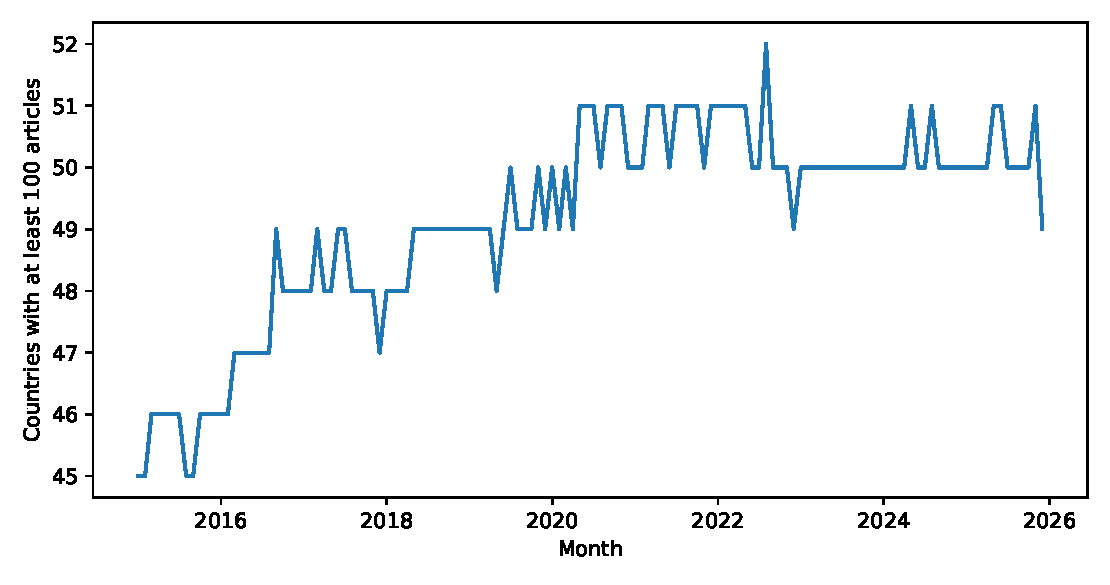
\includegraphics[width=0.82\textwidth]{Supplement_Figure_Coverage.pdf}
\caption{Monthly news-coverage diagnostic.}
\label{fig:coverage}
\end{figure}

A GRE archive-depth regression over the 6,488 country-months satisfying the 100-article criterion gives a log-article-volume coefficient of 0.103 with country fixed effects ($p=0.656$), and 0.100 with both country and month fixed effects ($p=0.713$). These diagnostics do not establish source representativeness but provide little evidence of a mechanical within-country relation between GRE and archive size.


\section{GDP-PPP data provenance and target-information audit}
The annual activity input is the exact series labelled ``GDP (PPP)-WEO'' in the author-supplied workbook \nolinkurl{GDP_Data_African_countries_AUTHOR_SUPPLIED_2026-09-13.xlsx}. The replication package freezes that workbook as supplied on 13 September 2026 and provides the cleaned country-year extract \nolinkurl{annual_gdp_ppp_weo_labeled_final_vintage_2015_2025.csv}. The workbook does not contain an IMF WEO publication-release identifier. The paper therefore treats the observations as final-vintage WEO-labelled data and does not claim that they reproduce the historical values available to forecasters at each origin.

The final-vintage monthly evaluation target is constructed by additive first-difference Denton. If $Y_c$ stacks annual benchmarks, $G_c^F$ stacks monthly values, $D$ is the first-difference operator, and $A$ maps months into annual sums, then
\[
\min_{G_c^F}(DG_c^F)'(DG_c^F)\quad\text{subject to}\quad AG_c^F=Y_c.
\]
The monthly values reaggregate exactly to the annual benchmarks. The realized target is $100[\log G^F_{ct}-\log G^F_{c,t-12}]$.

The critical information-timing distinction is that $G_c^F$ is \emph{not} supplied to the forecasting model as if it had been observed historically. For every forecast origin the script reconstructs a separate GDP history from annual benchmark years allowed by the release convention. Under the baseline May rule, annual year $y$ is not available until May of $y+1$. Denton is applied only through the most recent permitted annual year; months after that year and through the forecast origin are extrapolated at the log-monthly rate implied by the two most recent permitted annual totals. A target dated in year $y$ cannot enter the recursive training sample before May of $y+1$.

For example, at a January 2020 forecast origin the May rule permits annual benchmarks only through 2018, whereas a June 2020 origin permits 2019. The November sensitivity rule is more conservative: annual 2019 does not enter until November 2020. These rules prevent the 2020--2025 annual totals from mechanically shaping GDP lags before their assumed release dates.

The procedure still uses final-vintage values for annual years deemed released. It therefore does not remove revisions to previously released years. A genuine historical-vintage experiment would require archived country-level annual GDP vintages and release calendars for every economy. The revised manuscript states this limitation explicitly and uses the term ``publication-lagged final-vintage'' rather than ``real time'' or ``leakage-free.''


\section{Monte Carlo design and full simulation results}
The Monte Carlo exercise isolates target-information treatment from the institutional details of the African application. Each replication contains 54 economies from 2015 through 2025, annual GDP is temporally disaggregated with the same first-difference Denton operator used in the paper, and the benchmark conditions on three lags of twelve-month growth and country fixed effects. The retrospective design supplies the complete final-vintage Denton history; the publication-lagged design admits annual year $y$ only from May of $y+1$.

Three DGPs are reported. The \emph{current-state signal} is intentionally modest: the alternative variable measures the contemporaneous annual activity innovation with noise and contains no next-year innovation. It is calibrated to produce a small feasible short-horizon gain. The \emph{pure-noise placebo} replaces the signal with independent noise. The \emph{persistent-state stress} DGP raises annual persistence from 0.25 to 0.95 and increases the signal-to-noise ratio. It is chosen only to establish an existence result in which the retrospective design generates the same direction of 12-month reversal observed in the African data. It is not intended to match the full empirical horizon profile or identify the mechanism generating the empirical reversal.

\begin{table}[htbp]
\centering\scriptsize
\caption{Full Monte Carlo results across three DGPs}
\begin{tabular}{llrrr}
\toprule
DGP & Design & $h$ & Mean rel. RMSFE & Share $<1$\\
\midrule
Current-state & Retrospective & 1 & 1.0002 & 39.0\%\\
Current-state & Publication-lagged & 1 & 0.9969 & 97.7\%\\
Current-state & Retrospective & 3 & 1.0002 & 36.6\%\\
Current-state & Publication-lagged & 3 & 0.9973 & 96.5\%\\
Current-state & Retrospective & 6 & 1.0002 & 39.2\%\\
Current-state & Publication-lagged & 6 & 0.9987 & 84.6\%\\
Current-state & Retrospective & 12 & 1.0001 & 47.5\%\\
Current-state & Publication-lagged & 12 & 1.0025 & 47.6\%\\
\midrule
Persistent-state stress & Retrospective & 1 & 1.0042 & 12.3\%\\
Persistent-state stress & Publication-lagged & 1 & 0.8715 & 100.0\%\\
Persistent-state stress & Retrospective & 3 & 1.0024 & 10.1\%\\
Persistent-state stress & Publication-lagged & 3 & 0.8793 & 100.0\%\\
Persistent-state stress & Retrospective & 6 & 0.9990 & 73.2\%\\
Persistent-state stress & Publication-lagged & 6 & 0.9149 & 100.0\%\\
Persistent-state stress & Retrospective & 12 & 0.9962 & 90.2\%\\
Persistent-state stress & Publication-lagged & 12 & 1.0122 & 35.1\%\\
\midrule
Pure-noise placebo & Retrospective & 1 & 1.0002 & 34.5\%\\
Pure-noise placebo & Publication-lagged & 1 & 1.0001 & 42.0\%\\
Pure-noise placebo & Retrospective & 12 & 1.0001 & 43.1\%\\
Pure-noise placebo & Publication-lagged & 12 & 1.0015 & 46.5\%\\
\bottomrule
\end{tabular}
\end{table}

The two signal DGPs deliberately demonstrate different distortions. In the modest current-state DGP, retrospective final-vintage history largely suppresses feasible short-horizon value and does not create a 12-month gain. In the persistent-state stress DGP, the 12-month retrospective ratio falls to 0.9962 while the publication-lagged ratio rises to 1.0122, reproducing the direction of the empirical reversal. The stress design's much larger short-horizon effects show why it should not be read as an empirical calibration. The pair of simulations supports the general admissibility result: the sign and horizon location of the distortion depend on persistence, signal strength, and how the constructed target enters the benchmark. The placebo shows that the procedure does not mechanically turn unrelated noise into a useful predictor.

\section{Publication-lagged horizon profile}
The baseline results use the May release convention, 2015--2018 frozen text scaling, and January 2020--December 2025 target dates.
\begin{table}[htbp]
\centering\scriptsize
\caption{Full horizon profile under the May release convention}
\begin{tabular}{rrrrrrrr}
\toprule
$h$ & Benchmark RMSFE & GRE RMSFE & Rel. RMSFE & Rel. MAE & HAC CW $p$ & Two-way $p$ & Target months\\
\midrule
1 & 8.375 & 8.344 & 0.9964 & 0.9897 & 0.0006 & 0.053 & 72\\
3 & 8.493 & 8.473 & 0.9977 & 0.9928 & 0.041 & 0.084 & 72\\
6 & 8.588 & 8.620 & 1.0037 & 1.0028 & 0.878 & 0.869 & 72\\
12 & 19.264 & 19.357 & 1.0048 & 1.0122 & 0.905 & 0.872 & 72\\
\bottomrule
\end{tabular}
\end{table}

Holm correction across the four target-month HAC values gives adjusted $p=0.0023$ at one month and 0.122 at three months. The corresponding two-way adjusted values are 0.211 and 0.253. The result is therefore strongest under the target-month aggregation that directly preserves the contemporaneous country cross-section; the two-way calculation is a complementary, more conservative diagnostic in the baseline May specification.

\section{Release-month sensitivity}
\begin{table}[htbp]
\centering\scriptsize
\caption{One-month result under alternative annual-data release conventions}
\begin{tabular}{lrrrrrr}
\toprule
Release convention & Rel. RMSFE & Rel. MAE & HAC CW $p$ & Two-way $p$ & Bootstrap CW $p$ & Countries improved\\
\midrule
May of $y+1$ & 0.9964 & 0.9897 & 0.0006 & 0.053 & 0.037 & 33/54\\
July of $y+1$ & 0.9969 & 0.9894 & 0.0004 & 0.039 & 0.038 & 31/54\\
November of $y+1$ & 0.9973 & 0.9910 & 0.0001 & 0.030 & 0.019 & 32/54\\
\bottomrule
\end{tabular}
\end{table}

The direction of the one-month comparison survives progressively more conservative release rules. The raw point gain becomes smaller as annual information is withheld longer, but MAE remains approximately one percent below the benchmark and the dependence-aware test results remain favorable.

\section{Block-bootstrap uncertainty}
The moving-block bootstrap resamples 12-month target-date blocks and preserves the contemporaneous country cross-section. Under the May rule, the one-month raw RMSFE improvement is 0.362 percent. Across 5,000 replications, 82.6 percent of draws are positive, the 90 percent interval is approximately $[-0.34,1.31]$ percent, the 95 percent interval is $[-0.50,1.44]$ percent, and the one-sided bootstrap probability for a non-positive Clark--West mean is 0.037. Thus adjusted-loss inference is favorable, while the raw RMSFE improvement remains imprecisely estimated.

At 12 months, the corrected May-rule comparison is unfavorable: the actual RMSFE improvement is $-0.484$ percent and the bootstrap distribution is concentrated below zero. The revised paper therefore makes no long-horizon forecast-improvement claim.

\section{Domain-alignment comparison}
At one month, GRE is compared with broad AERI, Inflation Risk, and FX/External Risk under the identical publication-lagged benchmark.
\begin{table}[htbp]
\centering\scriptsize
\caption{Text comparators under the corrected one-month design}
\begin{tabular}{lrrrrr}
\toprule
Signal & Rel. RMSFE & Rel. MAE & HAC CW $p$ & Two-way $p$ & Raw-loss direction\\
\midrule
GRE & 0.9964 & 0.9897 & 0.0006 & 0.053 & Improves\\
Broad AERI & 1.0024 & 1.0020 & 0.0003 & 0.238 & Worsens\\
Inflation Risk & 1.0153 & 1.0225 & 1.000 & 0.992 & Worsens\\
FX/External Risk & 1.0003 & 0.9980 & $<0.001$ & 0.208 & Mixed / essentially neutral\\
\bottomrule
\end{tabular}
\end{table}

The Clark--West adjustment can be favorable even when unadjusted MSE is slightly higher, because it corrects the nested-model loss differential for the estimated augmentation. The manuscript therefore does not treat a small Clark--West $p$-value as sufficient evidence of improvement when relative RMSFE exceeds one. GRE is the only signal in this restricted set that reduces both RMSFE and MAE.


\section{Information-staleness and revision diagnostics}
The short-horizon interpretation in the main paper motivates two direct diagnostics. First, each release convention is split into forecast origins before and after the assumed annual-data release month. The results are:
\begin{table}[htbp]
\centering\scriptsize
\caption{One-month GRE performance by annual-information state}
\begin{tabular}{llrrrr}
\toprule
Release rule & State & Target months & Rel. RMSFE & Rel. MAE & HAC CW $p$\\
\midrule
May & Stale pre-release & 24 & 0.9925 & 0.9804 & 0.0008\\
May & Refreshed post-release & 48 & 0.9985 & 0.9947 & 0.0286\\
July & Stale pre-release & 36 & 0.9937 & 0.9815 & 0.0001\\
July & Refreshed post-release & 36 & 1.0010 & 0.9984 & 0.1432\\
November & Stale pre-release & 60 & 0.9975 & 0.9907 & 0.0005\\
November & Refreshed post-release & 12 & 0.9961 & 0.9926 & 0.0574\\
\bottomrule
\end{tabular}
\end{table}
The May and July conventions display the pattern expected if news is more useful when the latest annual benchmark is stale. The November split does not preserve the same RMSFE ordering and contains only 12 post-release target months. The pattern is therefore suggestive rather than definitive.

Second, the May, July, and November simulations are stacked and target-month loss improvement is regressed on the age, in months, of the annual information set while absorbing exact forecast-origin and release-convention effects. The information-age coefficient is 0.018 for raw squared-error improvement ($p=0.625$) and 0.023 for Clark--West adjusted loss ($p=0.539$). A separate country- and month-fixed-effect regression asks whether standardized GRE predicts the difference between final-vintage twelve-month growth at the forecast origin and the publication-lagged current-growth estimate. The GRE coefficient is $-0.073$ percentage points with two-way clustered $p=0.765$. These nulls rule out a strong claim that GRE mechanically forecasts subsequent statistical revisions.

\section{Article-level exact-text deduplication sensitivity}
A separately reconstructed article archive collapses exact decoded article bodies within each country-month before the AERI pillars are recomputed. The reconstruction removes 497,091 records, 2.33 percent of reconstructed article rows, including 186,379 exact copies appearing across different outlets. The resulting deduplicated Growth/Real Economy pillar is then standardized using the same 2015--2018 calibration period and re-entered into the corrected publication-lagged forecast design.

On 7,126 common country-months, original and exact-text-deduplicated GRE have Pearson correlation 0.9689, Spearman correlation 0.9806, and median within-country correlation 0.9990. Table 6 reports the one-month forecasting comparison.
\begin{table}[htbp]
\centering\scriptsize
\caption{Exact-text-deduplicated GRE forecast sensitivity}
\begin{tabular}{lrrrrr}
\toprule
Signal & Rel. RMSFE & Rel. MAE & HAC CW $p$ & Two-way $p$ & Forecast observations\\
\midrule
Original GRE, common sample & 0.9964 & 0.9897 & 0.0006 & 0.053 & 3,886\\
Exact-text-deduplicated GRE & 0.9969 & 0.9905 & 0.0017 & 0.068 & 3,886\\
\bottomrule
\end{tabular}
\end{table}
This exercise shows that repeated identical text is not responsible for the direction of the short-horizon result. It is deliberately narrower than a full alternative-classifier validation: the production lexicon, severity tiers, and emphasis coefficients are unchanged.

\section{Wide macroeconomic factor benchmark}
The earlier narrow factor diagnostic is replaced by a genuinely wide cross-country information set. At each origin we assemble up to 162 monthly macroeconomic series: publication-lagged GDP growth, inflation, and exchange-rate depreciation for each of 54 economies. Inflation and exchange-rate variables are lagged to reduce release-timing concerns. These supplied macro series are final-vintage and do not include archived release-vintage metadata, so the factor exercise is a data-rich robustness benchmark rather than a historical real-time-vintage reconstruction. The March 2016--December 2018 calibration window determines admissibility, standardization, and PCA loadings. Series with fewer than 24 calibration observations or negligible variance are removed, leaving 159. The number of factors is selected without reference to forecast loss: six factors are the minimum required to exceed 80 percent of calibration-sample variance, explaining 82.1 percent.

\begin{table}[htbp]
\centering\scriptsize
\caption{GRE against the wide factor-augmented benchmark at one month}
\resizebox{\textwidth}{!}{%
\begin{tabular}{lrrrrrr}
\toprule
Benchmark & Benchmark RMSFE & +GRE RMSFE & Rel. RMSFE & Rel. MAE & HAC CW $p$ & Two-way $p$\\
\midrule
Parsimonious publication-lagged AR & 8.375 & 8.344 & 0.9964 & 0.9897 & 0.0006 & 0.053\\
Wide factors; macro lag 1 month & 9.325 & 9.313 & 0.9987 & 0.9946 & 0.112 & 0.148\\
Wide factors; macro lag 2 months & 9.875 & 9.881 & 1.0006 & 0.9972 & 0.451 & 0.457\\
\bottomrule
\end{tabular}}
\end{table}
The factor benchmark is richer but less accurate in absolute RMSFE than the parsimonious AR benchmark. More importantly, GRE no longer provides statistically persuasive incremental information against the factor augmentation. This result is retained because it defines the boundary of the empirical claim: the short-horizon GRE evidence is benchmark-dependent.

\section{Cross-sectional dependence}
For the one-month benchmark forecast errors, the balanced diagnostic panel contains 53 countries and 72 target months. Mean pairwise error correlation is 0.442 and the Pesaran CD statistic is approximately 139.2. At three, six, and twelve months the corresponding mean pairwise correlations are approximately 0.392, 0.365, and 0.563. These values motivate target-month aggregation, cross-section-preserving block resampling, and the complementary two-way covariance calculation.

\section{Retrospective final-vintage audit}
An earlier working specification used the final-vintage Denton monthly series as both the realized target and the lagged GDP history supplied to the forecast model. That design yielded a 12-month relative RMSFE of 0.9961 and nominal Clark--West $p=0.033$. Because annual benchmarks through 2025 helped determine the final-vintage monthly path, this specification does not represent the information available at historical forecast origins. It is retained only as an audit diagnostic.

Under the corrected May-rule information set the 12-month relative RMSFE becomes 1.0048 with target-month HAC $p=0.905$. At one month, by contrast, relative RMSFE is 0.9964. The comparison demonstrates that target-information timing changes the substantive horizon conclusion and is the principal reason the revised paper no longer characterizes the earlier 12-month result as pseudo-out-of-sample evidence.

\section{Signal-construction reproducibility}
For article $i$, the signal contribution is
\[
Q_i=R_iG_iS_iW_i,
\qquad
W_i=\operatorname{clip}(1+0.5T_i+0.2L_i+0.3M_i,1,2),
\]
with country-month aggregation
\[
GRE_{ct}=\frac{100}{N_{ct}}\sum_{i\in\mathcal A_{ct}}Q_i.
\]
The production architecture fixes the scoring rule before forecast evaluation. Each article contributes at most once to a given domain regardless of repeated keyword mentions; keyword frequencies are retained for diagnostics rather than used as multiplicative domain weights. Method identifiers and input hashes are checked before new observations are joined to the historical series, limiting accidental mixing of incompatible scoring vintages. The replication folder includes \texttt{Scoring\_Documentation/GRE\_Scoring\_Specification.md}, which records the exact frozen economic-relevance lexicon, all eight domain dictionaries needed to reconstruct the multi-domain indicator, the Growth/Real Economy activation terms, severity-tier mappings, title cues, the 1,200-character body-length rule, and the emphasis coefficients. The frozen lexical dictionaries explicitly cover English, French, and Portuguese terms; no separate Arabic-script activation dictionary is present in the production rule supplied with the replication materials. Arabic-only text can therefore be under-detected, and no Arabic terms are retrofitted after forecast evaluation. The compact forecasting package contains the frozen monthly GRE series and source registries, while the full production article archive is maintained separately because of its size. The final replication bundle also contains a reconstructed exact-text-deduplicated pillar series generated from the frozen archive and used in the forecasting sensitivity reported above. This provides an article-level perturbation of the retained-record universe. It does not vary the frozen dictionaries, severity maps, or emphasis coefficients, so the paper does not claim invariance to alternative classification architectures.


\section{Country-level one-month results}
Thirty-three of 54 economies have one-month relative RMSFE below one under the May release convention. The median country ratio is 0.9911. The full set is reported below rather than summarized only by the pooled statistic.
\begin{longtable}{lrr}
\caption{Country-level one-month relative RMSFE under the May release rule}\label{tab:supp_country}\\
\toprule
Country & Relative RMSFE & Evaluation observations \\
\midrule
\endfirsthead
\toprule
Country & Relative RMSFE & Evaluation observations \\
\midrule
\endhead
Algeria & 1.0211 & 72 \\
Angola & 0.9518 & 72 \\
Benin & 0.8940 & 72 \\
Botswana & 0.9875 & 72 \\
Burkina-Faso & 1.0646 & 72 \\
Burundi & 1.0949 & 72 \\
Cameroon & 0.9028 & 72 \\
Cape Verde & 1.0120 & 72 \\
Central African Republic & 1.0749 & 72 \\
Chad & 0.9712 & 72 \\
Comoros & 1.0060 & 72 \\
Congo & 0.9229 & 72 \\
Congo DRC & 0.9703 & 72 \\
Djibouti & 1.1348 & 72 \\
Egypt & 1.0968 & 72 \\
Equatorial Guinea & 1.0011 & 72 \\
Eritrea & 0.9354 & 72 \\
Eswatini & 1.0157 & 72 \\
Ethiopia & 0.9954 & 72 \\
Gabon & 0.9940 & 72 \\
Gambia & 0.9907 & 72 \\
Ghana & 1.0726 & 72 \\
Guinea & 1.0232 & 72 \\
Guinea-Bissau & 0.9971 & 71 \\
Ivory Coast & 1.0174 & 72 \\
Kenya & 0.9187 & 72 \\
Lesotho & 1.1125 & 72 \\
Liberia & 0.9879 & 72 \\
Libya & 1.0116 & 72 \\
Madagascar & 0.8165 & 72 \\
Malawi & 0.9754 & 72 \\
Mali & 0.9323 & 72 \\
Mauritania & 0.9915 & 72 \\
Mauritius & 0.9369 & 72 \\
Morocco & 1.1275 & 72 \\
Mozambique & 0.9100 & 72 \\
Namibia & 1.0759 & 72 \\
Niger & 0.9897 & 72 \\
Nigeria & 0.9453 & 72 \\
Rwanda & 0.9846 & 72 \\
Sao Tome and Principe & 1.0252 & 72 \\
Senegal & 1.0604 & 72 \\
Seychelles & 1.0042 & 72 \\
Sierra Leone & 0.8933 & 72 \\
Somalia & 1.0423 & 72 \\
South Africa & 0.9321 & 72 \\
South Sudan & 0.9976 & 72 \\
Sudan & 0.9850 & 72 \\
Tanzania & 0.9521 & 72 \\
Togo & 0.9663 & 72 \\
Tunisia & 0.9962 & 72 \\
Uganda & 0.9798 & 72 \\
Zambia & 0.9838 & 72 \\
Zimbabwe & 0.9777 & 72 \\
\bottomrule
\end{longtable}

\section{Country universe}
\begin{longtable}{l}
\caption{Countries in the full GDP forecasting universe}\label{tab:supp_countries}\\
\toprule Country \\
\midrule\endfirsthead
\toprule Country \\
\midrule\endhead
Algeria \\
Angola \\
Benin \\
Botswana \\
Burkina-Faso \\
Burundi \\
Cameroon \\
Cape Verde \\
Central African Republic \\
Chad \\
Comoros \\
Congo \\
Congo DRC \\
Djibouti \\
Egypt \\
Equatorial Guinea \\
Eritrea \\
Eswatini \\
Ethiopia \\
Gabon \\
Gambia \\
Ghana \\
Guinea \\
Guinea-Bissau \\
Ivory Coast \\
Kenya \\
Lesotho \\
Liberia \\
Libya \\
Madagascar \\
Malawi \\
Mali \\
Mauritania \\
Mauritius \\
Morocco \\
Mozambique \\
Namibia \\
Niger \\
Nigeria \\
Rwanda \\
Sao Tome and Principe \\
Senegal \\
Seychelles \\
Sierra Leone \\
Somalia \\
South Africa \\
South Sudan \\
Sudan \\
Tanzania \\
Togo \\
Tunisia \\
Uganda \\
Zambia \\
Zimbabwe \\
\bottomrule
\end{longtable}


\end{document}
